% author Truong Nhan Nguyen
% created in 9/1/2022

\documentclass[tikz, border=10pt]{standalone}

\usepackage{tikz}
\usepackage{pgfmath}

\begin{document}
    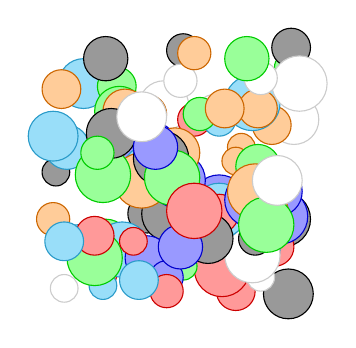
\begin{tikzpicture}
        % create a random list of colors: red, green, blue, orange, cyan, black, white
        \pgfmathdeclarerandomlist{color}{{red}{green}{blue}{orange}{cyan}{black}{white}}
        % repeat drawing circle
        \foreach \p in {1, 2, ..., 100}{
            % select randomly x coordinate
            \pgfmathrandominteger{\x}{1}{90}
            % select randomly y coordinate
            \pgfmathrandominteger{\y}{1}{90}
            % select randomly radius
            \pgfmathrandominteger{\r}{5}{10}
            % select randomly circle's color
            \pgfmathrandomitem{\c}{color}
            % construct circle with (x, y) and radius r
            \pgfpathcircle{\pgfpoint{+\x pt}{+\y pt}}{+\r pt}
            % set filling color
            \pgfsetfillcolor{\c!40!white}
            % set drawing color
            \pgfsetstrokecolor{\c!80!black}
            % draw circle and fill it with color
            \pgfusepath{stroke, fill}
        }
    \end{tikzpicture}
\end{document}